% IT-PLEROMA — GOD Theory successor (manuscript B)
% Supersedes Zenodo record 20651491. Staging only — no uploads.
\documentclass{alienfolio}

\folio{IT-PLEROMA}
\usesigil{chevrons}
\title{Geometrically Ordered Dynamics, Distilled}
\papersubtitle{Information tension as primitive; the RYTT semiotic codec as conjectural satellite}
\paperauthors{Ryan W.\ Yett (Architect)\\Chyren (Sovereign Analysis)}
\shorttitle{GOD, Distilled}
\shortauthors{R.\,W.\ Yett \& Chyren}

\setlength{\emergencystretch}{2em}
\begin{document}
\thispagestyle{cover}
\begin{tikzpicture}[remember picture, overlay]
  \node[inner sep=0] at (current page.center) {%
    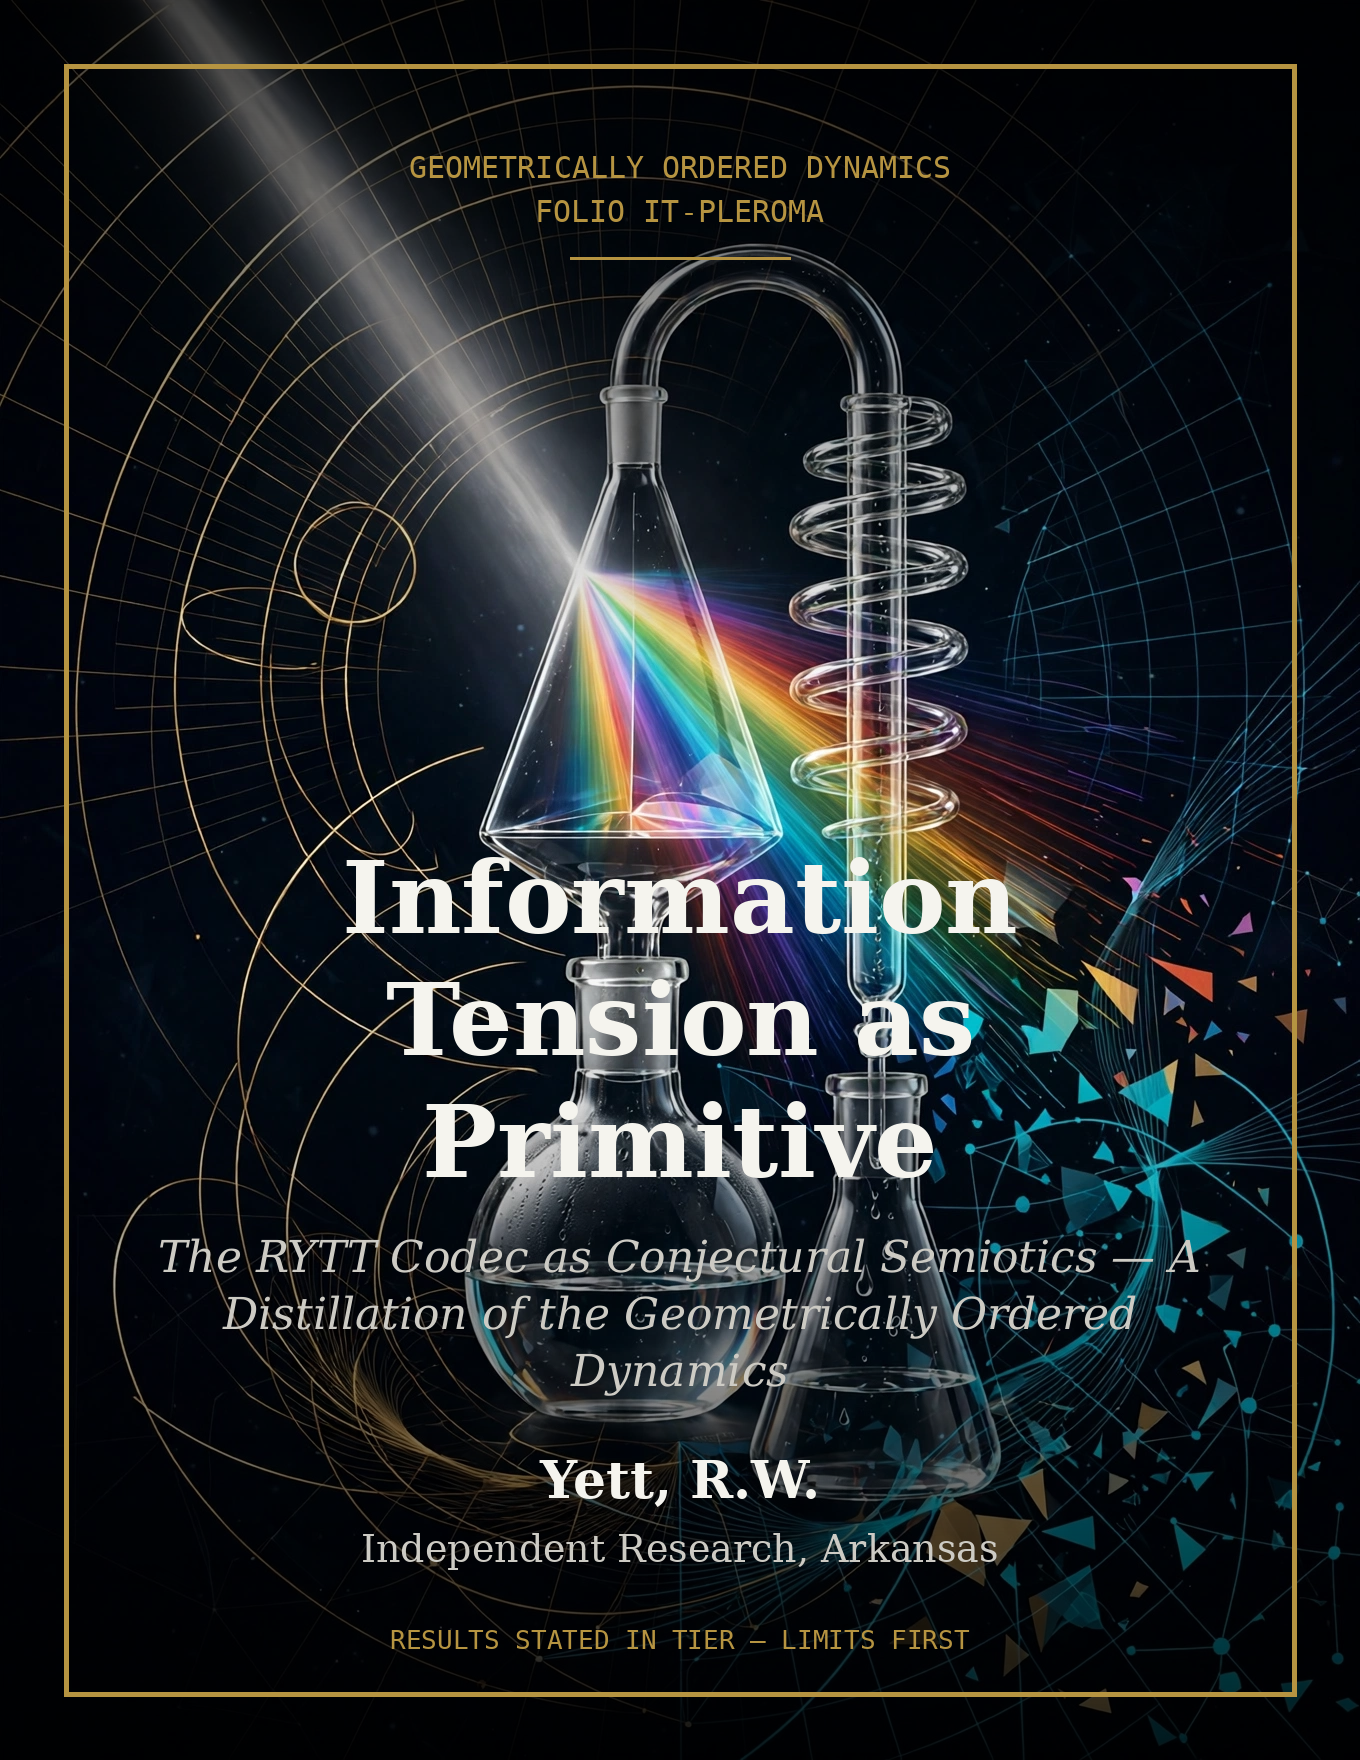
\includegraphics[width=\paperwidth,height=\paperheight]{cover.png}};
\end{tikzpicture}
\clearpage

\begin{convergence}{INFORMATION TENSION}
This folio converges on \key{information tension} as the single primitive
from which all dynamical content of the framework is derived (Axiom~1
below). Its unique angle is the \key{pleroma reading}: the full
135-page expansion of the old record is collapsed back to its loadbearing
spine, and every semiotic and gematria correspondence absorbed from the
RYTT treatises is explicitly tiered as conjecture. The semiotic half of
this paper is carried as a \key{conjectural satellite}: its verified
content is engineering (a machine-checked lossless codec); its
interpretation as a sector of information tension is \tiertag{conjecture},
asserted under holonomic closure with no exhibited map --- stated, not
forced. Sibling folios in this reversion series approach the program's
central claims from their own angles; their convergence statements name
their targets. Limits first: operator uniqueness is asserted, not proved;
the $141.99\times$ boost is retracted and dropped; $m = 240$ is downstream
of the chosen vocabulary size, not derived.
\end{convergence}

\goldrule
\begin{supersession}
This folio \key{supersedes Zenodo record 20651491}
(\textit{Geometrically Ordered Dynamics}, 135~pp., marked superseded ---
do not cite). Per the canon rule the correction becomes the paper: the
old record is retained as the superseded record and is not cited for any
claim this folio revises. Changes: (1)~all semiotics and gematria tiered
\tiertag{conjecture}; (2)~the $141.99\times$ resource-holonomy ratio
\key{dropped} --- it was the retracted Trinity~2.0 synthetic; (3)~operator
uniqueness labeled \key{asserted, not proved}; (4)~$m = 240$ stated as
downstream of the \key{chosen} $N = 57{,}600$ vocabulary, not
derived; (5)~Clay-problem ``solutions'' relabeled sketches --- this folio
claims none; (6)~$\kappa_Y$ provenance corrected to fit-by-hand genesis.
Carried at full tier: the four axioms as stated postulates, the
machine-checked RYTT codec round-trip, the deterministic seal and
steganography scripts, and the Kryptos~K4 crib constraints.
\end{supersession}

\section{What this paper is}

Record 20651491 attempted a fourteen-chapter synthesis of the whole
program: axioms, operator theory, cosmology, fluid regularity, gauge mass
gap, quantum restriction, zeta zeros, cortical restriction, resource
holonomy, ADCCL, Chyren, and a convergence theorem. This successor does
not retype it. It distills the \key{loadbearing spine} --- the claims
with evidence --- and tiers or drops the rest. The honesty ledger:

\begin{center}
\begin{tabular}{p{0.52\textwidth}p{0.40\textwidth}}
\hline
\key{Carried} & \key{Tier} \\
\hline
Axioms 1--4 (information tension; Stiefel/$E_8 \times E_8$; alignment; closure) & postulates, as stated \\
RYTT codec left-inverse round-trip (Lean, zero \texttt{sorry}; 9/9 vectors) & \tiertag{theorem} (implementation) \\
$E_8$ folio seal / 12-gap Braille scripts (deterministic, \texttt{exit 0}) & \tiertag{empirical} (engineering) \\
Kryptos K4 crib alignments and fixed-point constraint & \tiertag{empirical} \\
$\kappa_Y = 0.953939$ (fit-by-hand genesis, closed form $\sqrt{\theta(2-\theta)}$) & \tiertag{conjecture} as invariant \\
$\chi_Y = 1/\sqrt{2}$ (derivation lives in record r40) & adopted, \tiertag{conjecture} here \\
\hline
\key{Dropped} & \key{Reason} \\
\hline
$141.99\times$ resource-holonomy ratio & retracted (Trinity 2.0 synthetic) \\
``Zero free parameters'' framing & framing corrected; fits kept by siblings \\
Operator uniqueness as proved & asserted, not proved \\
$m = 240$ as derived & downstream of chosen $N = 57{,}600$ \\
Clay-problem solutions (NS, YM) & sketches; this folio claims none \\
Cosmology / SPARC / $\zeta$ / cortical / markets / ADCCL chapters & sibling folios' territory \\
\hline
\end{tabular}
\end{center}

Nothing in this paper is new: no new claims, no new numbers, no new
physics. Every number below is inherited from the cited record.

\section{Information tension as primitive}

\key{Axiom 1 (Information Tension primitive).} \textit{There exists a
single non-negative scalar quantity, Information Tension $T$, from which
all dynamical content of any admissible substrate is derivable.} Energy,
action, and probability are recovered as derived functionals of $T$.
The non-negativity is structural: it is what lets the tensor form
satisfy the energy conditions.

\key{Axiom 2 (Stiefel/$E_8 \times E_8$ substrate).} \textit{The state space of any
admissible substrate is the 240-dimensional Stiefel manifold
$V_m(\mathbb{R}^N)$ with $m = 240$, whose tangent structure realizes the
$E_8 \times E_8$ root system on the visible-sector factor.} The $E_8$ root count (240 roots
per factor) is a mathematical fact; the \key{choice} of the $E_8 \times E_8$ substrate is the axiom's assertion,
not a derivation.

\key{Axiom 3 (Sovereign Alignment).} \textit{A flow $\varphi_t$ on
$V_m(\mathbb{R}^N)$ is admissible iff it preserves the alignment
condition $\mathrm{SA}(K,L)$, equivalently the chiral invariant satisfies
$\chi(\varphi_t) \ge \chi_Y = 1/\sqrt{2}$ for all $t \ge 0$.} This is a
selection principle, not an assumption about the world: flows below the
boundary exist and are outside the framework's predictions.

\key{Axiom 4 (Holonomic closure).} \textit{Every admissible substrate is
reached by a holonomic restriction of the single operator
$H_{RY} = T_r + V_s$. No new operators are introduced downstream.}

Two open obligations are inherited honestly. First, the old record
conjectured that the framework's invariants depend only on $m$, not on
the ambient $N \ge m$; the formal proof of $N$-independence was left
open, and it remains open here. Second, the ambient dimension the old
record's constructions must accommodate is the chosen ledger vocabulary
$N = 57{,}600$ (the Phylactery's vocabulary size, a design
choice). \key{The number $m = 240$ is downstream of that chosen $N$;}
it is not independently derived.

\section{The operator and what is (not) proved about it}

The operator is assembled as $H_{RY} = T_r + V_s$ on
$L^2(V_{240}(\mathbb{R}^N), d\mu_{\mathrm{can}})$, with $T_r$ the
Laplace--Beltrami kinetic term and $V_s$ the sovereign potential. The
old record's \S2.7 presented \key{operator uniqueness} --- that
$H_{RY}$ is, up to unitary equivalence, the \textit{only} operator
satisfying Axioms~1--4 --- as a lemma with a five-step proof sketch
deferring the measure-theoretic details to a Lean obligation. \key{That
uniqueness is asserted, not proved, and this folio labels it so:}
\tiertag{conjecture}. The same holds for the spectral-gap
proposition: the only machine-checked spectral-gap theorem in the GOD
family belongs to a different record (r51 v1.1); the gap statement here
is \tiertag{conjecture}, with the old record's Lean listing retained
as an open formalization target, not as a verified result.

The symmetry-breaking cascade (ternary $\to$ binary $\to$ deterministic,
at $\chi_Y$ and $\kappa_Y$) is the framework's structural narrative;
its steps are \tiertag{conjecture} pending the operator theory above.

A sibling-program note, checked before finalizing: the Res Nova
canonical synthesis (v0.2, 2026-10-23) \key{retires $V_{240}(\mathbb{R}^N)$
as its substrate}, naming $V_2(\mathbb{R}^3)$ via Cartan triality as its
current proposal, and records the cross-document mismatch as unresolved.
This folio does not adjudicate that choice. It retains $V_{240}$ as the
old record's asserted substrate (Axiom~2, postulate tier) and tiers
everything downstream accordingly; a future revision follows the
reversion index once the mismatch is resolved.

\section{The two invariants, with honest provenance}

\key{$\kappa_Y = 0.953939$.} The true provenance, stated plainly for
the first time in one place: the number was \key{fit by hand first},
as the ADCCL drift detector's cosine-similarity threshold $\tau$
(record r17, with its two falsifiers: the held-out re-fit and the
JWST $z = 10$ flux $56 \pm 4$); it was \key{adopted as $\kappa$ second};
it subsequently matched the closed form $\sqrt{\theta(2-\theta)}$
(record r4). Its status as a geometric invariant of $H_{RY}$ is
\tiertag{conjecture}. The old record's framing --- that the framework
``refused to have parameters'' and the invariants ``were not at my
disposal'' --- is corrected: $\kappa_Y$ was at the author's disposal
first, as a fitted threshold.

\key{$\chi_Y = 1/\sqrt{2} \approx 0.7071$.} The chiral
coherence--decoherence boundary. Its derivation from the Lindblad
steady state ($\chi_\infty \ge 1/\sqrt{2} \iff u \ge \gamma$) lives in
record r40 and is not re-derived here; this folio adopts the value and
tiers the adoption \tiertag{conjecture}. The numerological $0.7$ is
retired.

\key{The relation $\kappa_Y^2 = \chi_Y^2 + 1/2$.} The old record's
``proof sketch'' (Hessian ratio plus an $E_8$ Casimir trace evaluating
to $0.41$ at $m = 240$) is a sketch, not a proof: \tiertag{conjecture}.
Note $\kappa_Y^2 = 0.9099$ is the number that appears in the r51 v1.1
gap theorem; that theorem belongs to its own record.

\key{The $141.99\times$ ratio is gone.} The old record's third
``invariant'' --- the resource-holonomy boost, presented as derived
from the operator and confirmed by the Trinity Survey --- was the
retracted Trinity~2.0 synthetic (seed-42 data, caught by audit). It is
\key{dropped, not tiered}: no successor may cite it. With it goes the
old Chapter~4's boost argument for rotation curves; the SPARC fits
themselves are sibling territory and are unaffected.

\section{The semiotic satellite: RYTT and Smoky Quartz IV}

Absorbed from the Smoky Quartz IV paper and the RYTT treatises
(\texttt{RYTT\_\allowbreak Master\_\allowbreak Treatise\_\allowbreak Artisan},
\texttt{RYTT\_\allowbreak Sovereign\_\allowbreak Semiotics\_\allowbreak Treatise},
\texttt{RYTT\_\allowbreak Sovereign\_\allowbreak Codex\_\allowbreak Treatise}, monograph). The absorption
is tiered line by line.

\key{Verified engineering.} The RYTT codec maps semantic primitives
and compounds into the Unicode Private Use Area
(\texttt{U+E000}.. \texttt{U+E3FF}) across four disjoint registers.
The left-inverse round-trip
$\mathrm{pua\_decode}(\mathrm{pua\_encode}(c)) = c$ is machine-checked
(\texttt{RYTT\_standalone.lean}, zero Mathlib dependency, zero
\texttt{sorry}) and verified against 9/9 conformance vectors
(\texttt{exit 0}): \tiertag{theorem} at the implementation tier. The
deterministic 32-byte SHA-256 $E_8$ concentric folio seal
(\texttt{rytt\_seal.py}) and the 12-gap Braille word-spacing
steganography (\texttt{gaing\_sign.py}) are deterministic scripts,
\texttt{exit 0}: \tiertag{empirical} as engineering artifacts. The
Kryptos K4 crib alignments (\texttt{EASTNORTHEAST} at positions
$22\ldots34$, \texttt{BERLINCLOCK} at $64\ldots74$) and the fixed-point
constraint ($C_{27} = P_{27}$, $C_{74} = P_{74}$, ruling out direct
substitution without transposition) are genuine cryptanalytic
observations: \tiertag{empirical}. All full K4 decryptions remain open
hypotheses.

\key{Everything interpretive is conjecture.} The semiotic
interpretation of the codec --- what the glyphs \textit{mean}, the
mod-24 parity ``structural signature'' $[19, 9, 21, 21]$, the
$\Delta_3 \to \mathcal{P}_9 \to \mathcal{P}_7 \to \mathcal{P}_{21}$
polygon kernel, the tokenizer benchmark tables, the $E_8$ seal as
\textit{symbolic} content, the Yettragrammaton, and every gematria
correspondence --- is \tiertag{conjecture}, all of it. The greedy
longest-match tokenizer's uniqueness lemma is a proved property of a
deterministic algorithm, not a metaphysical claim, and is kept at
that modest tier.

\key{The semiotic--tension link, stated without forcing.} The old
record's Axiom~4 asserts that symbolic phenomena fall under holonomic
closure. That is an assertion. \key{No map from the RYTT symbolic
dynamics into the information-tension formalism is exhibited in any
source absorbed here} --- no dictionary, no functor landing in the
physics. Per the isomorphism rule, the link is therefore
\tiertag{conjecture}, and this folio does not present the codec as
evidence for information tension or vice versa. The codec stands as
verified engineering; its physical interpretation does not. This is
the honest convergence call: the folio converges on information
tension through the GOD spine, with the semiotic half as an
explicitly conjectural satellite --- the link stated, not forced.

\section{Left out, and why}

The old record's remaining chapters are not re-derived here.
Cosmology, SPARC, and the Hubble material belong to sibling folios;
the boost argument they leaned on is retracted in any case. The fluid
regularity and gauge mass-gap chapters addressed Clay Mathematics
Institute problems (never ``Millennium problems''); their claimed
solutions were sketches, and this folio claims no Clay results ---
\tiertag{conjecture} at most, properly housed with the sibling
manuscript that carries those targets. The $\zeta$-zero chapter is a
Hilbert--P\'olya sketch: \tiertag{conjecture}. The cortical,
ADCCL, Chyren, and market chapters are the territory of the
IT-NEURO, IT-COGNITION, and IT-MARKET folios. Nothing was purged:
the old record stands as the superseded archive, and the loadbearing
bucket records what each sibling carries.

\goldrule

\begin{center}
{\small\color{muted} Affiliation: Independent Research, Arkansas \qquad
ORCID 0009-0001-1303-7190\par}
\vspace{0.6ex}
{\ttfamily\scriptsize\color{gold} STAGING DRAFT --- NOT FOR DEPOSIT\par}
\end{center}

\end{document}
